
% Default to the notebook output style

    


% Inherit from the specified cell style.




    
\documentclass{article}

    
    
    \usepackage{graphicx} % Used to insert images
    \usepackage{adjustbox} % Used to constrain images to a maximum size 
    \usepackage{color} % Allow colors to be defined
    \usepackage{enumerate} % Needed for markdown enumerations to work
    \usepackage{geometry} % Used to adjust the document margins
    \usepackage{amsmath} % Equations
    \usepackage{amssymb} % Equations
    \usepackage{eurosym} % defines \euro
    \usepackage[mathletters]{ucs} % Extended unicode (utf-8) support
    \usepackage[utf8x]{inputenc} % Allow utf-8 characters in the tex document
    \usepackage{fancyvrb} % verbatim replacement that allows latex
    \usepackage{grffile} % extends the file name processing of package graphics 
                         % to support a larger range 
    % The hyperref package gives us a pdf with properly built
    % internal navigation ('pdf bookmarks' for the table of contents,
    % internal cross-reference links, web links for URLs, etc.)
    \usepackage{hyperref}
    \usepackage{longtable} % longtable support required by pandoc >1.10
    \usepackage{booktabs}  % table support for pandoc > 1.12.2
    

    
    
    \definecolor{orange}{cmyk}{0,0.4,0.8,0.2}
    \definecolor{darkorange}{rgb}{.71,0.21,0.01}
    \definecolor{darkgreen}{rgb}{.12,.54,.11}
    \definecolor{myteal}{rgb}{.26, .44, .56}
    \definecolor{gray}{gray}{0.45}
    \definecolor{lightgray}{gray}{.95}
    \definecolor{mediumgray}{gray}{.8}
    \definecolor{inputbackground}{rgb}{.95, .95, .85}
    \definecolor{outputbackground}{rgb}{.95, .95, .95}
    \definecolor{traceback}{rgb}{1, .95, .95}
    % ansi colors
    \definecolor{red}{rgb}{.6,0,0}
    \definecolor{green}{rgb}{0,.65,0}
    \definecolor{brown}{rgb}{0.6,0.6,0}
    \definecolor{blue}{rgb}{0,.145,.698}
    \definecolor{purple}{rgb}{.698,.145,.698}
    \definecolor{cyan}{rgb}{0,.698,.698}
    \definecolor{lightgray}{gray}{0.5}
    
    % bright ansi colors
    \definecolor{darkgray}{gray}{0.25}
    \definecolor{lightred}{rgb}{1.0,0.39,0.28}
    \definecolor{lightgreen}{rgb}{0.48,0.99,0.0}
    \definecolor{lightblue}{rgb}{0.53,0.81,0.92}
    \definecolor{lightpurple}{rgb}{0.87,0.63,0.87}
    \definecolor{lightcyan}{rgb}{0.5,1.0,0.83}
    
    % commands and environments needed by pandoc snippets
    % extracted from the output of `pandoc -s`
    \DefineVerbatimEnvironment{Highlighting}{Verbatim}{commandchars=\\\{\}}
    % Add ',fontsize=\small' for more characters per line
    \newenvironment{Shaded}{}{}
    \newcommand{\KeywordTok}[1]{\textcolor[rgb]{0.00,0.44,0.13}{\textbf{{#1}}}}
    \newcommand{\DataTypeTok}[1]{\textcolor[rgb]{0.56,0.13,0.00}{{#1}}}
    \newcommand{\DecValTok}[1]{\textcolor[rgb]{0.25,0.63,0.44}{{#1}}}
    \newcommand{\BaseNTok}[1]{\textcolor[rgb]{0.25,0.63,0.44}{{#1}}}
    \newcommand{\FloatTok}[1]{\textcolor[rgb]{0.25,0.63,0.44}{{#1}}}
    \newcommand{\CharTok}[1]{\textcolor[rgb]{0.25,0.44,0.63}{{#1}}}
    \newcommand{\StringTok}[1]{\textcolor[rgb]{0.25,0.44,0.63}{{#1}}}
    \newcommand{\CommentTok}[1]{\textcolor[rgb]{0.38,0.63,0.69}{\textit{{#1}}}}
    \newcommand{\OtherTok}[1]{\textcolor[rgb]{0.00,0.44,0.13}{{#1}}}
    \newcommand{\AlertTok}[1]{\textcolor[rgb]{1.00,0.00,0.00}{\textbf{{#1}}}}
    \newcommand{\FunctionTok}[1]{\textcolor[rgb]{0.02,0.16,0.49}{{#1}}}
    \newcommand{\RegionMarkerTok}[1]{{#1}}
    \newcommand{\ErrorTok}[1]{\textcolor[rgb]{1.00,0.00,0.00}{\textbf{{#1}}}}
    \newcommand{\NormalTok}[1]{{#1}}
    
    % Define a nice break command that doesn't care if a line doesn't already
    % exist.
    \def\br{\hspace*{\fill} \\* }
    % Math Jax compatability definitions
    \def\gt{>}
    \def\lt{<}
    % Document parameters
    \title{Homework 7}
    \author{Roly Vicar\'ia \\ STAT 500 Summer 2015}     
    

    % Pygments definitions
    
\makeatletter
\def\PY@reset{\let\PY@it=\relax \let\PY@bf=\relax%
    \let\PY@ul=\relax \let\PY@tc=\relax%
    \let\PY@bc=\relax \let\PY@ff=\relax}
\def\PY@tok#1{\csname PY@tok@#1\endcsname}
\def\PY@toks#1+{\ifx\relax#1\empty\else%
    \PY@tok{#1}\expandafter\PY@toks\fi}
\def\PY@do#1{\PY@bc{\PY@tc{\PY@ul{%
    \PY@it{\PY@bf{\PY@ff{#1}}}}}}}
\def\PY#1#2{\PY@reset\PY@toks#1+\relax+\PY@do{#2}}

\expandafter\def\csname PY@tok@gd\endcsname{\def\PY@tc##1{\textcolor[rgb]{0.63,0.00,0.00}{##1}}}
\expandafter\def\csname PY@tok@gu\endcsname{\let\PY@bf=\textbf\def\PY@tc##1{\textcolor[rgb]{0.50,0.00,0.50}{##1}}}
\expandafter\def\csname PY@tok@gt\endcsname{\def\PY@tc##1{\textcolor[rgb]{0.00,0.27,0.87}{##1}}}
\expandafter\def\csname PY@tok@gs\endcsname{\let\PY@bf=\textbf}
\expandafter\def\csname PY@tok@gr\endcsname{\def\PY@tc##1{\textcolor[rgb]{1.00,0.00,0.00}{##1}}}
\expandafter\def\csname PY@tok@cm\endcsname{\let\PY@it=\textit\def\PY@tc##1{\textcolor[rgb]{0.25,0.50,0.50}{##1}}}
\expandafter\def\csname PY@tok@vg\endcsname{\def\PY@tc##1{\textcolor[rgb]{0.10,0.09,0.49}{##1}}}
\expandafter\def\csname PY@tok@m\endcsname{\def\PY@tc##1{\textcolor[rgb]{0.40,0.40,0.40}{##1}}}
\expandafter\def\csname PY@tok@mh\endcsname{\def\PY@tc##1{\textcolor[rgb]{0.40,0.40,0.40}{##1}}}
\expandafter\def\csname PY@tok@go\endcsname{\def\PY@tc##1{\textcolor[rgb]{0.53,0.53,0.53}{##1}}}
\expandafter\def\csname PY@tok@ge\endcsname{\let\PY@it=\textit}
\expandafter\def\csname PY@tok@vc\endcsname{\def\PY@tc##1{\textcolor[rgb]{0.10,0.09,0.49}{##1}}}
\expandafter\def\csname PY@tok@il\endcsname{\def\PY@tc##1{\textcolor[rgb]{0.40,0.40,0.40}{##1}}}
\expandafter\def\csname PY@tok@cs\endcsname{\let\PY@it=\textit\def\PY@tc##1{\textcolor[rgb]{0.25,0.50,0.50}{##1}}}
\expandafter\def\csname PY@tok@cp\endcsname{\def\PY@tc##1{\textcolor[rgb]{0.74,0.48,0.00}{##1}}}
\expandafter\def\csname PY@tok@gi\endcsname{\def\PY@tc##1{\textcolor[rgb]{0.00,0.63,0.00}{##1}}}
\expandafter\def\csname PY@tok@gh\endcsname{\let\PY@bf=\textbf\def\PY@tc##1{\textcolor[rgb]{0.00,0.00,0.50}{##1}}}
\expandafter\def\csname PY@tok@ni\endcsname{\let\PY@bf=\textbf\def\PY@tc##1{\textcolor[rgb]{0.60,0.60,0.60}{##1}}}
\expandafter\def\csname PY@tok@nl\endcsname{\def\PY@tc##1{\textcolor[rgb]{0.63,0.63,0.00}{##1}}}
\expandafter\def\csname PY@tok@nn\endcsname{\let\PY@bf=\textbf\def\PY@tc##1{\textcolor[rgb]{0.00,0.00,1.00}{##1}}}
\expandafter\def\csname PY@tok@no\endcsname{\def\PY@tc##1{\textcolor[rgb]{0.53,0.00,0.00}{##1}}}
\expandafter\def\csname PY@tok@na\endcsname{\def\PY@tc##1{\textcolor[rgb]{0.49,0.56,0.16}{##1}}}
\expandafter\def\csname PY@tok@nb\endcsname{\def\PY@tc##1{\textcolor[rgb]{0.00,0.50,0.00}{##1}}}
\expandafter\def\csname PY@tok@nc\endcsname{\let\PY@bf=\textbf\def\PY@tc##1{\textcolor[rgb]{0.00,0.00,1.00}{##1}}}
\expandafter\def\csname PY@tok@nd\endcsname{\def\PY@tc##1{\textcolor[rgb]{0.67,0.13,1.00}{##1}}}
\expandafter\def\csname PY@tok@ne\endcsname{\let\PY@bf=\textbf\def\PY@tc##1{\textcolor[rgb]{0.82,0.25,0.23}{##1}}}
\expandafter\def\csname PY@tok@nf\endcsname{\def\PY@tc##1{\textcolor[rgb]{0.00,0.00,1.00}{##1}}}
\expandafter\def\csname PY@tok@si\endcsname{\let\PY@bf=\textbf\def\PY@tc##1{\textcolor[rgb]{0.73,0.40,0.53}{##1}}}
\expandafter\def\csname PY@tok@s2\endcsname{\def\PY@tc##1{\textcolor[rgb]{0.73,0.13,0.13}{##1}}}
\expandafter\def\csname PY@tok@vi\endcsname{\def\PY@tc##1{\textcolor[rgb]{0.10,0.09,0.49}{##1}}}
\expandafter\def\csname PY@tok@nt\endcsname{\let\PY@bf=\textbf\def\PY@tc##1{\textcolor[rgb]{0.00,0.50,0.00}{##1}}}
\expandafter\def\csname PY@tok@nv\endcsname{\def\PY@tc##1{\textcolor[rgb]{0.10,0.09,0.49}{##1}}}
\expandafter\def\csname PY@tok@s1\endcsname{\def\PY@tc##1{\textcolor[rgb]{0.73,0.13,0.13}{##1}}}
\expandafter\def\csname PY@tok@kd\endcsname{\let\PY@bf=\textbf\def\PY@tc##1{\textcolor[rgb]{0.00,0.50,0.00}{##1}}}
\expandafter\def\csname PY@tok@sh\endcsname{\def\PY@tc##1{\textcolor[rgb]{0.73,0.13,0.13}{##1}}}
\expandafter\def\csname PY@tok@sc\endcsname{\def\PY@tc##1{\textcolor[rgb]{0.73,0.13,0.13}{##1}}}
\expandafter\def\csname PY@tok@sx\endcsname{\def\PY@tc##1{\textcolor[rgb]{0.00,0.50,0.00}{##1}}}
\expandafter\def\csname PY@tok@bp\endcsname{\def\PY@tc##1{\textcolor[rgb]{0.00,0.50,0.00}{##1}}}
\expandafter\def\csname PY@tok@c1\endcsname{\let\PY@it=\textit\def\PY@tc##1{\textcolor[rgb]{0.25,0.50,0.50}{##1}}}
\expandafter\def\csname PY@tok@kc\endcsname{\let\PY@bf=\textbf\def\PY@tc##1{\textcolor[rgb]{0.00,0.50,0.00}{##1}}}
\expandafter\def\csname PY@tok@c\endcsname{\let\PY@it=\textit\def\PY@tc##1{\textcolor[rgb]{0.25,0.50,0.50}{##1}}}
\expandafter\def\csname PY@tok@mf\endcsname{\def\PY@tc##1{\textcolor[rgb]{0.40,0.40,0.40}{##1}}}
\expandafter\def\csname PY@tok@err\endcsname{\def\PY@bc##1{\setlength{\fboxsep}{0pt}\fcolorbox[rgb]{1.00,0.00,0.00}{1,1,1}{\strut ##1}}}
\expandafter\def\csname PY@tok@mb\endcsname{\def\PY@tc##1{\textcolor[rgb]{0.40,0.40,0.40}{##1}}}
\expandafter\def\csname PY@tok@ss\endcsname{\def\PY@tc##1{\textcolor[rgb]{0.10,0.09,0.49}{##1}}}
\expandafter\def\csname PY@tok@sr\endcsname{\def\PY@tc##1{\textcolor[rgb]{0.73,0.40,0.53}{##1}}}
\expandafter\def\csname PY@tok@mo\endcsname{\def\PY@tc##1{\textcolor[rgb]{0.40,0.40,0.40}{##1}}}
\expandafter\def\csname PY@tok@kn\endcsname{\let\PY@bf=\textbf\def\PY@tc##1{\textcolor[rgb]{0.00,0.50,0.00}{##1}}}
\expandafter\def\csname PY@tok@mi\endcsname{\def\PY@tc##1{\textcolor[rgb]{0.40,0.40,0.40}{##1}}}
\expandafter\def\csname PY@tok@gp\endcsname{\let\PY@bf=\textbf\def\PY@tc##1{\textcolor[rgb]{0.00,0.00,0.50}{##1}}}
\expandafter\def\csname PY@tok@o\endcsname{\def\PY@tc##1{\textcolor[rgb]{0.40,0.40,0.40}{##1}}}
\expandafter\def\csname PY@tok@kr\endcsname{\let\PY@bf=\textbf\def\PY@tc##1{\textcolor[rgb]{0.00,0.50,0.00}{##1}}}
\expandafter\def\csname PY@tok@s\endcsname{\def\PY@tc##1{\textcolor[rgb]{0.73,0.13,0.13}{##1}}}
\expandafter\def\csname PY@tok@kp\endcsname{\def\PY@tc##1{\textcolor[rgb]{0.00,0.50,0.00}{##1}}}
\expandafter\def\csname PY@tok@w\endcsname{\def\PY@tc##1{\textcolor[rgb]{0.73,0.73,0.73}{##1}}}
\expandafter\def\csname PY@tok@kt\endcsname{\def\PY@tc##1{\textcolor[rgb]{0.69,0.00,0.25}{##1}}}
\expandafter\def\csname PY@tok@ow\endcsname{\let\PY@bf=\textbf\def\PY@tc##1{\textcolor[rgb]{0.67,0.13,1.00}{##1}}}
\expandafter\def\csname PY@tok@sb\endcsname{\def\PY@tc##1{\textcolor[rgb]{0.73,0.13,0.13}{##1}}}
\expandafter\def\csname PY@tok@k\endcsname{\let\PY@bf=\textbf\def\PY@tc##1{\textcolor[rgb]{0.00,0.50,0.00}{##1}}}
\expandafter\def\csname PY@tok@se\endcsname{\let\PY@bf=\textbf\def\PY@tc##1{\textcolor[rgb]{0.73,0.40,0.13}{##1}}}
\expandafter\def\csname PY@tok@sd\endcsname{\let\PY@it=\textit\def\PY@tc##1{\textcolor[rgb]{0.73,0.13,0.13}{##1}}}

\def\PYZbs{\char`\\}
\def\PYZus{\char`\_}
\def\PYZob{\char`\{}
\def\PYZcb{\char`\}}
\def\PYZca{\char`\^}
\def\PYZam{\char`\&}
\def\PYZlt{\char`\<}
\def\PYZgt{\char`\>}
\def\PYZsh{\char`\#}
\def\PYZpc{\char`\%}
\def\PYZdl{\char`\$}
\def\PYZhy{\char`\-}
\def\PYZsq{\char`\'}
\def\PYZdq{\char`\"}
\def\PYZti{\char`\~}
% for compatibility with earlier versions
\def\PYZat{@}
\def\PYZlb{[}
\def\PYZrb{]}
\makeatother


    % Exact colors from NB
    \definecolor{incolor}{rgb}{0.0, 0.0, 0.5}
    \definecolor{outcolor}{rgb}{0.545, 0.0, 0.0}



    
    % Prevent overflowing lines due to hard-to-break entities
    \sloppy 
    % Setup hyperref package
    \hypersetup{
      breaklinks=true,  % so long urls are correctly broken across lines
      colorlinks=true,
      urlcolor=blue,
      linkcolor=darkorange,
      citecolor=darkgreen,
      }
    % Slightly bigger margins than the latex defaults
    
    \geometry{verbose,tmargin=1in,bmargin=1in,lmargin=1in,rmargin=1in}
    
    

    \begin{document}
    
    
    \maketitle
    
    

    
    \subsubsection{Question 1.}\label{question-1.}

    \begin{Verbatim}[commandchars=\\\{\}]
{\color{incolor}In [{\color{incolor}1}]:} \PY{c}{\PYZsh{} 1a) 95\PYZpc{} confidence interval}
        \PY{o}{\PYZpc{}}\PY{k}{run} mystats
        \PY{n}{reading\PYZus{}speed} \PY{o}{=} \PY{p}{[}\PY{l+m+mi}{5}\PY{p}{,} \PY{l+m+mi}{7}\PY{p}{,} \PY{l+m+mi}{15}\PY{p}{,} \PY{l+m+mi}{10}\PY{p}{,} \PY{l+m+mi}{8}\PY{p}{,} \PY{l+m+mi}{7}\PY{p}{,} \PY{l+m+mi}{10}\PY{p}{,} \PY{l+m+mi}{11}\PY{p}{,} \PY{l+m+mi}{9}\PY{p}{,} \PY{l+m+mi}{13}\PY{p}{,} \PY{l+m+mi}{10}\PY{p}{,} \PY{l+m+mi}{8}\PY{p}{,} \PY{l+m+mi}{11}\PY{p}{,} \PY{l+m+mi}{8}\PY{p}{,} \PY{l+m+mi}{10}\PY{p}{,} \PY{l+m+mi}{8}\PY{p}{,} \PY{l+m+mi}{7}\PY{p}{,} \PY{l+m+mi}{6}\PY{p}{,} \PY{l+m+mi}{11}\PY{p}{,} \PY{l+m+mi}{8}\PY{p}{]}
        \PY{n}{t\PYZus{}interval}\PY{p}{(}\PY{n}{reading\PYZus{}speed}\PY{p}{,} \PY{n}{conf}\PY{o}{=}\PY{o}{.}\PY{l+m+mi}{95}\PY{p}{)}
\end{Verbatim}

            \begin{Verbatim}[commandchars=\\\{\}]
{\color{outcolor}Out[{\color{outcolor}1}]:} (7.9749195160742703, 10.225080483925728)
\end{Verbatim}
        
    \textbf{1b) } Probability plot 
    
    \begin{figure}[h]
 \centering
 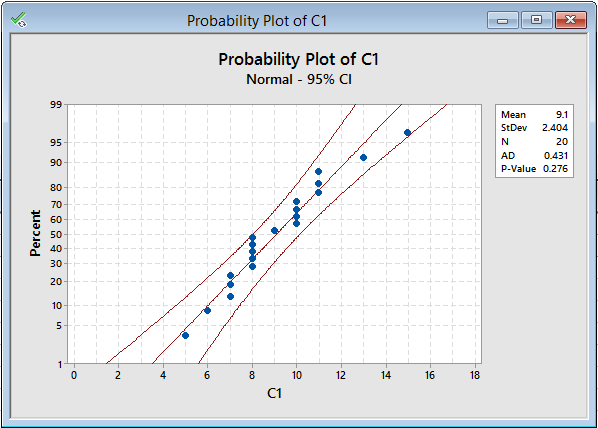
\includegraphics[scale=.8]{./images/probplot2.png}
 % probplot2.png: 598x428 pixel, 96dpi, 15.82x11.32 cm, bb=0 0 448 321
\end{figure}


    \textbf{1c) } The interval indicates that there is 95\% chance that the true
population mean lies within the range 7.975 and 10.225. And if we
repeatedly sample 20 students and compute this interval, there is a 95\%
chance that the intervals would contain the mean $\mu$. Stated another
way, about 95\% of those intervals would contain $\mu$.

    \begin{Verbatim}[commandchars=\\\{\}]
{\color{incolor}In [{\color{incolor}3}]:} \PY{c}{\PYZsh{} 1d) 97\PYZpc{} confidence interval}
        \PY{n}{t\PYZus{}interval}\PY{p}{(}\PY{n}{reading\PYZus{}speed}\PY{p}{,} \PY{n}{conf}\PY{o}{=}\PY{o}{.}\PY{l+m+mi}{97}\PY{p}{)}
\end{Verbatim}

            \begin{Verbatim}[commandchars=\\\{\}]
{\color{outcolor}Out[{\color{outcolor}3}]:} (7.8391247336019489, 10.36087526639805)
\end{Verbatim}
        
    Changing from a 95\% confidence interval to a 97\% confidence interval
merely gives us a wider interval (2.25 vs 2.522), thus also a less
precise interval. We can say that there is a 97\% chance that the
population mean falls within the range 7.839 to 10.361.

    \subsubsection{Question 2.}\label{question-2.}

    \begin{Verbatim}[commandchars=\\\{\}]
{\color{incolor}In [{\color{incolor}4}]:} \PY{c}{\PYZsh{} Using formula to compute 95\PYZpc{} confidence interval}
        \PY{n}{x\PYZus{}bar} \PY{o}{=} \PY{l+m+mf}{9.10}
        \PY{n}{s} \PY{o}{=} \PY{l+m+mf}{2.404}
        \PY{n}{n} \PY{o}{=} \PY{l+m+mi}{20}
        
        \PY{n}{t} \PY{o}{=} \PY{n}{stats}\PY{o}{.}\PY{n}{t}\PY{p}{(}\PY{n}{n} \PY{o}{\PYZhy{}} \PY{l+m+mi}{1}\PY{p}{)}
        \PY{p}{(}\PY{n}{x\PYZus{}bar} \PY{o}{\PYZhy{}} \PY{n}{t}\PY{o}{.}\PY{n}{ppf}\PY{p}{(}\PY{o}{.}\PY{l+m+mi}{975}\PY{p}{)}\PY{o}{*}\PY{p}{(}\PY{n}{s}\PY{o}{/}\PY{n}{np}\PY{o}{.}\PY{n}{sqrt}\PY{p}{(}\PY{n}{n}\PY{p}{)}\PY{p}{)}\PY{p}{,} \PY{n}{x\PYZus{}bar} \PY{o}{+} \PY{n}{t}\PY{o}{.}\PY{n}{ppf}\PY{p}{(}\PY{o}{.}\PY{l+m+mi}{975}\PY{p}{)}\PY{o}{*}\PY{p}{(}\PY{n}{s}\PY{o}{/}\PY{n}{np}\PY{o}{.}\PY{n}{sqrt}\PY{p}{(}\PY{n}{n}\PY{p}{)}\PY{p}{)}\PY{p}{)}
\end{Verbatim}

            \begin{Verbatim}[commandchars=\\\{\}]
{\color{outcolor}Out[{\color{outcolor}4}]:} (7.9748933669665369, 10.225106633033462)
\end{Verbatim}
        
    \subsubsection{Question 3.}\label{question-3.}

\begin{enumerate}
\def\labelenumi{\alph{enumi})}
\item
  A point estimate for the mean time would be $\bar{y} = 27.6$
\item
  Standard deviation of point estimate is
  $s /\sqrt{n} = 3.7 / \sqrt{34} = 0.6345$
\end{enumerate}

    \begin{Verbatim}[commandchars=\\\{\}]
{\color{incolor}In [{\color{incolor}5}]:} \PY{c}{\PYZsh{} 3c) 95\PYZpc{} confidence interval}
        \PY{n}{y\PYZus{}bar} \PY{o}{=} \PY{l+m+mf}{27.6}
        \PY{n}{s} \PY{o}{=} \PY{l+m+mf}{3.7}
        \PY{n}{n} \PY{o}{=} \PY{l+m+mi}{34}
        
        \PY{n}{t} \PY{o}{=} \PY{n}{stats}\PY{o}{.}\PY{n}{t}\PY{p}{(}\PY{n}{n} \PY{o}{\PYZhy{}}\PY{l+m+mi}{1}\PY{p}{)}
        \PY{p}{(}\PY{n}{y\PYZus{}bar} \PY{o}{\PYZhy{}} \PY{n}{t}\PY{o}{.}\PY{n}{ppf}\PY{p}{(}\PY{o}{.}\PY{l+m+mi}{975}\PY{p}{)}\PY{o}{*}\PY{p}{(}\PY{n}{s}\PY{o}{/}\PY{n}{np}\PY{o}{.}\PY{n}{sqrt}\PY{p}{(}\PY{n}{n}\PY{p}{)}\PY{p}{)}\PY{p}{,} \PY{n}{y\PYZus{}bar} \PY{o}{+} \PY{n}{t}\PY{o}{.}\PY{n}{ppf}\PY{p}{(}\PY{o}{.}\PY{l+m+mi}{975}\PY{p}{)}\PY{o}{*}\PY{p}{(}\PY{n}{s}\PY{o}{/}\PY{n}{np}\PY{o}{.}\PY{n}{sqrt}\PY{p}{(}\PY{n}{n}\PY{p}{)}\PY{p}{)}\PY{p}{)}
\end{Verbatim}

            \begin{Verbatim}[commandchars=\\\{\}]
{\color{outcolor}Out[{\color{outcolor}5}]:} (26.309008968635599, 28.890991031364404)
\end{Verbatim}
        
    The office manager should interpret this as saying that there is a 95\%
chance that the true mean resolution time falls within the range 26.3 to
28.9 minutes. Or that the manager can be 95\% confident that cases are
being resolved between 26.3 and 28.9 minutes.

    \subsubsection{Question 4.}\label{question-4.}

\begin{enumerate}
\def\labelenumi{\alph{enumi})}
\itemsep1pt\parskip0pt\parsep0pt
\item
  True
\item
  True
\item
  False
\item
  False
\end{enumerate}

    \subsubsection{Question 5.}\label{question-5.}

    \begin{Verbatim}[commandchars=\\\{\}]
{\color{incolor}In [{\color{incolor}9}]:} \PY{c}{\PYZsh{} 5a) 99\PYZpc{} confidence interval}
        \PY{n}{reading\PYZus{}time} \PY{o}{=} \PY{n}{np}\PY{o}{.}\PY{n}{array}\PY{p}{(}\PY{p}{[}\PY{l+m+mi}{25}\PY{p}{,} \PY{l+m+mi}{18}\PY{p}{,} \PY{l+m+mi}{27}\PY{p}{,} \PY{l+m+mi}{29}\PY{p}{,} \PY{l+m+mi}{20}\PY{p}{,} \PY{l+m+mi}{19}\PY{p}{,} \PY{l+m+mi}{16}\PY{p}{,} \PY{l+m+mi}{24}\PY{p}{,} \PY{l+m+mi}{37}\PY{p}{,} \PY{l+m+mi}{21}\PY{p}{,} \PY{l+m+mi}{24}\PY{p}{,} \PY{l+m+mi}{19}\PY{p}{,} \PY{l+m+mi}{20}\PY{p}{,} \PY{l+m+mi}{28}\PY{p}{,} \PY{l+m+mi}{31}\PY{p}{,} \PY{l+m+mi}{22}\PY{p}{]}\PY{p}{)}
        
        \PY{n}{y\PYZus{}bar} \PY{o}{=} \PY{n}{reading\PYZus{}time}\PY{o}{.}\PY{n}{mean}\PY{p}{(}\PY{p}{)}
        \PY{n}{n} \PY{o}{=} \PY{n+nb}{len}\PY{p}{(}\PY{n}{reading\PYZus{}time}\PY{p}{)}
        \PY{n}{s} \PY{o}{=} \PY{n}{np}\PY{o}{.}\PY{n}{sqrt}\PY{p}{(}\PY{n+nb}{sum}\PY{p}{(}\PY{p}{[}\PY{p}{(}\PY{n}{y} \PY{o}{\PYZhy{}} \PY{n}{y\PYZus{}bar}\PY{p}{)} \PY{o}{*}\PY{o}{*} \PY{l+m+mi}{2} \PY{k}{for} \PY{n}{y} \PY{o+ow}{in} \PY{n}{reading\PYZus{}time}\PY{p}{]}\PY{p}{)} \PY{o}{/} \PY{p}{(}\PY{n}{n} \PY{o}{\PYZhy{}} \PY{l+m+mi}{1}\PY{p}{)}\PY{p}{)}
        
        \PY{n}{t} \PY{o}{=} \PY{n}{stats}\PY{o}{.}\PY{n}{t}\PY{p}{(}\PY{n}{n} \PY{o}{\PYZhy{}} \PY{l+m+mi}{1}\PY{p}{)}
        \PY{p}{(}\PY{n}{y\PYZus{}bar} \PY{o}{\PYZhy{}} \PY{n}{t}\PY{o}{.}\PY{n}{ppf}\PY{p}{(}\PY{o}{.}\PY{l+m+mi}{995}\PY{p}{)}\PY{o}{*}\PY{p}{(}\PY{n}{s}\PY{o}{/}\PY{n}{np}\PY{o}{.}\PY{n}{sqrt}\PY{p}{(}\PY{n}{n}\PY{p}{)}\PY{p}{)}\PY{p}{,} \PY{n}{y\PYZus{}bar} \PY{o}{+} \PY{n}{t}\PY{o}{.}\PY{n}{ppf}\PY{p}{(}\PY{o}{.}\PY{l+m+mi}{995}\PY{p}{)}\PY{o}{*}\PY{p}{(}\PY{n}{s}\PY{o}{/}\PY{n}{np}\PY{o}{.}\PY{n}{sqrt}\PY{p}{(}\PY{n}{n}\PY{p}{)}\PY{p}{)}\PY{p}{)}
\end{Verbatim}

            \begin{Verbatim}[commandchars=\\\{\}]
{\color{outcolor}Out[{\color{outcolor}9}]:} (19.657179514587956, 27.842820485412044)
\end{Verbatim}
        
    \textbf{5b) } The interval above is applicable for the population of
reading speeds of third graders in the large school district.

    \textbf{5c) } Based on the interval from part (a) we can say that we are
95\% confident that the average third grader reading speed is between
19.7 and 27.8 minutes.

    \subsubsection{Question 6.}\label{question-6.}

    \begin{Verbatim}[commandchars=\\\{\}]
{\color{incolor}In [{\color{incolor}7}]:} \PY{c}{\PYZsh{} number of renters needed in survey}
        \PY{n}{z} \PY{o}{=} \PY{n}{stats}\PY{o}{.}\PY{n}{norm}\PY{p}{(}\PY{p}{)}\PY{o}{.}\PY{n}{ppf}\PY{p}{(}\PY{o}{.}\PY{l+m+mi}{96}\PY{p}{)}
        \PY{n}{E} \PY{o}{=} \PY{l+m+mi}{97}
        \PY{n}{sigma} \PY{o}{=} \PY{p}{(}\PY{l+m+mi}{1500} \PY{o}{\PYZhy{}} \PY{l+m+mi}{45}\PY{p}{)} \PY{o}{/} \PY{l+m+mf}{4.}
        
        \PY{n}{np}\PY{o}{.}\PY{n}{ceil}\PY{p}{(}\PY{p}{(}\PY{p}{(}\PY{n}{z} \PY{o}{*}\PY{o}{*} \PY{l+m+mi}{2}\PY{p}{)} \PY{o}{*} \PY{p}{(}\PY{n}{sigma} \PY{o}{*}\PY{o}{*} \PY{l+m+mi}{2}\PY{p}{)}\PY{p}{)} \PY{o}{/} \PY{p}{(}\PY{n}{E} \PY{o}{*}\PY{o}{*} \PY{l+m+mi}{2}\PY{p}{)}\PY{p}{)}
\end{Verbatim}

            \begin{Verbatim}[commandchars=\\\{\}]
{\color{outcolor}Out[{\color{outcolor}7}]:} 44.0
\end{Verbatim}
        
    \subsubsection{Question 7.}\label{question-7.}

    \begin{Verbatim}[commandchars=\\\{\}]
{\color{incolor}In [{\color{incolor}8}]:} \PY{c}{\PYZsh{} number of renters needed in survey}
        \PY{c}{\PYZsh{} for 98\PYZpc{} confidence interval}
        
        \PY{n}{z} \PY{o}{=} \PY{n}{stats}\PY{o}{.}\PY{n}{norm}\PY{p}{(}\PY{p}{)}\PY{o}{.}\PY{n}{ppf}\PY{p}{(}\PY{o}{.}\PY{l+m+mi}{99}\PY{p}{)}
        \PY{n}{np}\PY{o}{.}\PY{n}{ceil}\PY{p}{(}\PY{p}{(}\PY{p}{(}\PY{n}{z} \PY{o}{*}\PY{o}{*} \PY{l+m+mi}{2}\PY{p}{)} \PY{o}{*} \PY{p}{(}\PY{n}{sigma} \PY{o}{*}\PY{o}{*} \PY{l+m+mi}{2}\PY{p}{)}\PY{p}{)} \PY{o}{/} \PY{p}{(}\PY{n}{E} \PY{o}{*}\PY{o}{*} \PY{l+m+mi}{2}\PY{p}{)}\PY{p}{)}
\end{Verbatim}

            \begin{Verbatim}[commandchars=\\\{\}]
{\color{outcolor}Out[{\color{outcolor}8}]:} 77.0
\end{Verbatim}
        

    % Add a bibliography block to the postdoc
    
    
    
    \end{document}
